\documentclass[chaparabic,ee,ms,12pt,oneandhalf]{metu}
\usepackage{appendix}
\usepackage{mathptmx}
\usepackage{caption}
\usepackage{amsmath}
\usepackage{times}
\author{Kadir Çimenci}
\title{Dynamic Formation Control with Heterogenous Mobile Robots}
\turkishtitle{Heterojen Robotlarla Dinamik Formasyon Kontrolü}
\date{June 2016}
\director[prof]{xxx}
\headofdept[prof]{Gönül Turhan Sayhan}
\supervisor[prof]{Aydan Erkmen}
\cosupervisor[assistprof]{xx}
\departmentofsupervisor{Electrical and Electronics Engineering Department, METU}
\departmentofcosupervisor{Electrical and Electronics Engineering Department, METU.}
\committeememberi[prof]{İsmail Hakkı Toroslu}
\affiliationi{Computer Engineering Department, METU}
\committeememberii[prof]{Ali H. Doğru}
\affiliationii{Computer Engineering Department, METU}
\committeememberiii[assocprof]{Pınar Karagöz}
\affiliationiii{Computer Engineering Department, METU}
\committeememberiv[assistprof]{Selim Temizer}
\affiliationiv{Computer Engineering Department, METU}
\committeememberv[assistprof]{Aykut Erdem}
\affiliationv{Computer Engineering Department, Hacettepe University}
\keywords{Multi Agent Systems, Formation Control, Localization, Mesh Network}
\anahtarklm{Çok Elemanlı Sistemler, Formasyon Kontrolü, Konumlama, Örgün Ağlar}

\abstract{Formation control in robotics is a growing topic where mainly research works are geared towards heterogenous swarm colonies under decentralized control or heterogenous colonies where some centralization is considered. In swarm works where decentralization is applied, it is nevertheless assumed that the agents are capable of getting global information about the whole swarm.Moreover in the literature, formation control is generally done for known fixed shapes that can be defined mathematically. However no dynamically changing shapes are envisaged and no shape transitions are clearly handled in those works. We attempt to bring a clear impact to the literature by focusing our thesis work on tracking and realising formation shapes under dynamically changing formation shape demands. Furthermore,in our thesis work, we focus on robot colonies composed of heterogeneous robots of different dynamics and sensory capabilities under decentralized dynamically changing formation control. These robots are able furthermore, to just posess local mutual interactions only with their closeby neighboring agents. Using communications with those neighbors, all agents are being able to acquire graph theoretically, information about the whole colony. Simulations in our work will be generated using the Gazebo environment modeling a rough territory. Hardware applications of our approach will also be developed.}

\oz{Formasyon kontrolü robotik alanında heterojen robot kolonilerinin merkezi yönetici birimler olmadan ya da yerel merkezi birimleri barındıran topolojilerle kontrolü konularına yönelik büyüyen bir araştırma alanıdır. Merkezi yönetim birimlerinin olmadığı robot sürüsü çalışmalarında ne yazık ki her üyenin, koloniye mensup diğer üyelerin tüm verilerine erişebildiği varsayımı yapılmaktadır.Öte yandan, literatürde formasyon kontrolü genellikle matematiksel olarak ifade edilebilen basit geometrik şekillerle yapılmaktadır. Bununla birlikte bu çalışmalarda, dinamik olarak değişen şekiller ve bu şekiller arasında formasyon geçişleri konusu yeterli olarak ele alınmamaktadır. Bu çalışma kapsamında dinamik olarak değişen şekiller için formasyon kontrolü sağlayarak literatüre katkıda bulunmayı hedefliyoruz. Öte yandan bu tez çalışmamızda, farklı dinamiklere ve sensör yetkinliklerine sahip heterojen robot kolonileri kullanarak dinamik formasyon kontrolü problemini merkezi karar verici birimlerin olmadığı bir topolojide ele alacağız. Çalışma kapsamında ele alınan kolonilerdeki tüm robotlar yalnızca kendilerine en yakın komşu üyelerle yerel etkileşimlerde bulunabileceklerdir. Komşularıyla etkileşimde bulunan üyeler, konsensus koordinat sistemi ve koloninin geri kalanı hakkında bilgi sahibi olabileceklerdir. Çalışmamız kapsamında simülasyonlar Gazebo ortamında üç boyutlu düzgün olmayan araziler modellenerek yapılacaktır. Ayrıca donanımsal gerçeklemeler içeren çalışmalar da yapılacaktır.} 

\dedication{\textit{To my family and people who are reading this page}}
 
\acknowledgments{
TODO
}


\usepackage[pdftex]{hyperref}
\usepackage[all]{hypcap}
\usepackage{todonotes}
\usepackage{graphicx}
\graphicspath{ {./images/} }
\usepackage{rotating}
\usepackage{xy} 
\usepackage{booktabs}
\usepackage{pifont}
\usepackage{color}
\usepackage{listings}
\usepackage{pdfpages}
\usepackage{array}
\newcolumntype{M}{>{\centering\arraybackslash}m{\dimexpr.25\linewidth-2\tabcolsep}}
\renewcommand\lstlistingname{XChor Language - }
\def\lstlistingautorefname{XChorCode.}
\lstset{
language = java,
basicstyle=\small,
numbers=left,
numbersep=10pt,
numberstyle=\tiny\color{black},
stepnumber=1,
tabsize=2,
showspaces=false, 
frame=single,
breaklines=true,
escapeinside=~~
}
\usepackage{float}
\restylefloat{figure}
\newcommand{\tab}{\hspace*{2em}}
\DeclareGraphicsExtensions{.pdf,.png,.jpg}

\begin{document}

% Preliminaries
\begin{preliminaries}
% If you are willing to use any custom stuff before Chapters, put it here
% Such as List of Abbreviations
% Check the abbreviations.tex for a template list of abbreviations

\begin{theglossary}{LONGESTABBRV}
\item[ABBRV] Abbreviation
\end{theglossary}

% End of Preliminaries
\end{preliminaries}
%   
% Latex content Goes Here 
% 
%

% CHAPTER 1

\chapter{INTRODUCTION}
\label{chp:introduction}

This thesis work focuses on dynamic adaptation to achieve changes in formation of swarms consisting of heterogeneous mobile robots. The term of swarm has a meaning \cite{4}, a large group of locally interacting individuals with common goals. 

Self organizing swarm researches and its applications are generally inspired from the biological systems existing in the nature. Behaviours of complex biological systems remained unresolved for a long time, until recent researches that showed individuals with supple functionalities can achieve complex tasks by cooperation \cite{2}. Biological systems (such as colonies of ants) have simple behaviours but they can accomplish very complicated collective tasks in nature quite impossible to be achieved solely by individual capabilities. Beni \cite{1} describes this collaboration of members as follows:

Collaborative robot network is not just an agglomeration of robots, they have essential characteristics, which are found in swarms of insects, that is, decentralised control, which does not require synchronisation, and individuals which are simple and (quasi) identical.

Properties of swarm robotics systems that make them unique are the simplicity of individuals, restricted sensing and communication capabilities, collaborative achievement of complex tasks, robustness and decentralization of control capabilities \cite{6}.

Swarm robotics has been studied to produce different collective behaviours to solve different tasks such as as aggregation , pattern formation , self-assembly and morphogenesis , object clustering, assembling and construction , collective search$\&$rescue and exploration , coordinated motion , collective transportation , self-deployment , foraging and others\cite{5}. Dorigo and Trianni \cite{7} are studied on controllers for aggregation of coordinated motion of the identical mobile robots called swarm-bots. Their implementation has a centralized structure in which a decision maker assigns roles to individual agents. In our work, each agent is responsible to reach global consensus on the final positions in formation which increase the robustness of the system against to individual erroneous decisions. Hou et al. is focused on controlling of a swarm within a dynamically changing formation \cite{8}. In their work, it is needed to describe a global objective function which requires analytical expression of the desired formation shape. But it may not be possible to define the desired formation shape with analytical expressions in real world applications. In this thesis work, the solution does not require the analytical expressions of the desired formation shape.  Ganesh and Lisa introduced two new strategies for collective search and exploration of fields with swarm intelligence \cite{9}. Their implementation requires a central controller to manage the individuals and this type of solution has a single point of failure system characteristic because of the dependence on single decision maker agent.   Chaimowicz and Campos proposed a new methodology which is based on a dynamic role assignment mechanism in which the robots cooperate with each other and they demonstrate this method in a cooperative transportation task \cite{10}. Their work implements a leader follower structure in which following agents has no impact on the global consensus of the swarm. This approach depends on the decisions of an individual agent and an erroneous decisions of this individual may cause the failure of whole swarm. 

There are lots of studies related with different problems in swarm robotics literature as discussed briefly. In this thesis project, we are focused on dynamic pattern formation control of swarms consist of heterogeneous robots. All agents contribute on the decision process and they collaborate to minimize the total displacement while achieving the desired formation shape. 

\section{Problem Definition}
In this thesis work, we aimed to design a formation control system with heterogeneous robots and dynamically changing complex shapes. Desired formation shapes for real time applications, such as covering an area or a search$\&$rescue operation, may not be simple geometrical shapes with analytical expressions. The solution which does not require a mathematical definition of the desired formation shape is more suitable for these type of applications. On the other hand, this formation shape may be dynamically changing to meet the requirements of the task in real time. 

In literature, formation control systems generally include a decision making process which is executed by an individual agent or a central server. This kind of approach creates a single point of failure system and this ruler may cause a failure for the whole swarm by making a mistake. In this work, it is aimed to implement a solution in which each member of the swarm contributes on the decisions and global consensus of the swarm.

Formation control systems which are implemented with swarms composed of homogeneous agents cannot achieve special tasks which requires different functionalities of individual agents. In this work, we have focused on implementing a solution with a swarm consisting of heterogeneous agents with different capabilities. 

In this work, the main idea is to propose a complete design solution to a dynamically changing formation system, including a local positioning and formation control system. Formation control system heavily depends on the position data of individual agents in the workspace. Since it is expected to have high number of agents in the environment due to the nature of a swarm, the agents are assumed to have simple structures with low capabilities including lack of certain types of sensors. On the other hand, for indoor applications it will not be possible to use satellite dependent positioning systems on agents \cite{19}. Even if a positioning solution provided for an indoor application by different methods including visual feedback(by image processing), RSS(received signal strength) etc. , it is not possible to implement this solution for each single agent in the environment due to the increasing complexity and the costs by the number of agents. In literature, formation control systems are generally designed with the assumption of the positions of each agent is known exactly. To propose a complete solution for the formation control problem, it is required to implement a localization solution for the agents to provide the corrected positions in the workspace which will be used by the formation control system. This localization process must implement a solution to correct the position data of the agents within an maximum error bound. This error bound is determined by the requirements of the formation control problem. 

\section{Motivation}
The formation control problem is defined as the collaboration of a group of agents towards maintaining a formation with a certain shape \cite{12}. It focuses on leading the individual agents of a swarm to perform  collective tasks including shape generation and formation reconfiguration while traversing a trajectory avoiding collisions. These kind of tasks are achieved with a large group of simple robots  that can cooperate with each other. Formation control of multi agent systems  is an actively growing research field.

Swarms which are used in formation control systems, can be composed of homogeneous or heterogeneous agents according to the requirements of the problem. The usage of the homogeneous agents increases the total impact and the coverage of the system in the environment. This kind of a swarm has an increased redundancy and is capable of resuming the current task in case of failures of some of the agents during mission. On the other hand, a swarm composed of heterogeneous agents has different capabilities of the agents. This kind of a system can be used in tasks which requires different functionalities has to be performed individually or simultaneously.

In real world applications there may be need for different  functionalities to achieve some specific tasks. If this is the case, one solution may be to design a sophisticated robot which includes all required capabilities for this task. In this scenario, this robot will be the single point of failure in the system and if robustness is a  vital feature for this solution, some redundant robots have to be added to the system. It is clear that the design of such an advanced robot and hold its redundant backups in the system will increase the cost of the solution. In swarm robotics concept, one of the approaches related with the usage of the heterogeneous agents is to gather some different types of simple mobile robots which have their own specific functionalities to achieve a collective task rather than designing an advanced robot for the solution \cite{99}. With this approach, the robustness of the system is increased, costs are reduced down and the reusability of the individual members of the swarm for other tasks is provided.  A project named Swarmanoid which is funded by European Commission, has an objective to implement and control of a novel distributed robotic system. The system is designed with heterogeneous, dynamically connected, small autonomous robots called foot-bots , hand-bots and eye-bots where foot-bots are responsible to transport the required materials(including other types of robots) to a specific task area and hand-bots are responsible for operations to be handled with their manipulators and eye-bots are responsible of observations and reconnaissance on the workspace. This project implements a system which has a leader follower structure in which a decision maker agent assign different tasks and roles to the other members of the swarm. Wrong decisions or the failure of this decision maker may prevent the whole swarm to achieve the desired task. In this thesis work, we have focused on a system in which each agent is responsible to contribute on the decision process.

\begin{figure}[H]
\caption{A Robot Team Consists of Eyebot, Handbot and Footbot Agents \cite{99}}
\centering
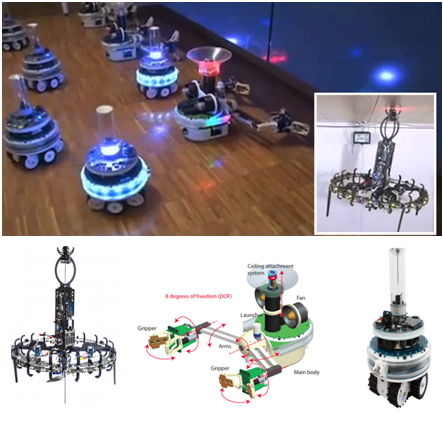
\includegraphics[scale = 1]{eyebot}
\end{figure} 
\newpage
A swarm which is composed with same type of homogeneous agents can be used to increase the total impact and the energy of an individual agent. This kind of a system can be used in missions like coverage, search and  reconnaissance etc.  Martin and Kilberg have worked on formation control and formation tracking of  microsatellites to achieve continuous coverage and improved capability. They also mentioned that small formations will reduce the fuel consumption for propulsion and expand the sensing capabilities of microsatellites \cite{15}.

\begin{figure}[H]
\caption{Sparse Aperture Formation of Micro Satellites \cite{15}}
\centering
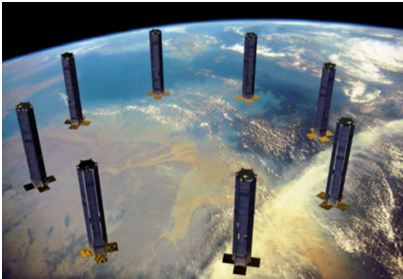
\includegraphics[scale = 1]{Satellite}
\end{figure} 

Formation control solutions has lots of usage areas such as coverage missions, security patrols and search$\&$rescue in hazardous environments etc.\cite{13}. For missions related with area coverage and reconnaissance, a group of autonomous vehicles may be required to keep in a specified formation \cite{13}.  

There are some hardware implementations to test the related formation control algorithms in real time applications. Since the formation control problem requires lots of agents in a swarm, these works have a common point of providing agents with minimal costs and sensor capabilities. The Kilobot Project from Harvard university have released their agents with the name of Kilobots and they have teams which are working on different formation control problems with Kilobots \cite{98}.

\begin{figure}[H]
\caption{Formation Control with Kilobots \cite{98}}
\centering
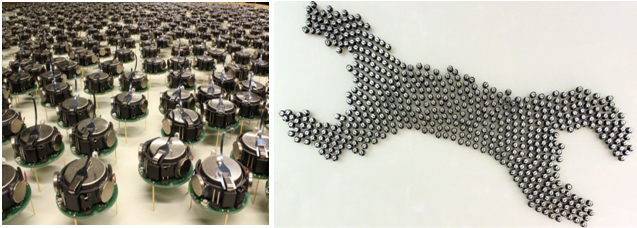
\includegraphics[scale = 0.70]{kilobot}
\end{figure}

These micro robots have a great reusability for different types of formation control problems  and they have biological inspiration from the nature in the sense of individual simplicity and power of collective behaviours. Common feature of these projects, they implement formation control systems with swarms composed of homogeneous agents. In real world applications, complex tasks may require different functionalities which can be provided by different types of robots. In our work, we have focused on implementing a formation control system with heterogeneous agents.

\begin{figure}[H]
\captionsetup{format=hang,justification=centerfirst}
\caption{
A) Swarm Robot Project from Universities of Stuttgart \cite{97}  \\
B) Colias Project from Lincoln University and Tsinghua University\cite{96}\\
C) Marx bot developed at EPFL\cite{95} \\
D)Swarm bots project conducted by  European Commission \cite{94}}

\centering
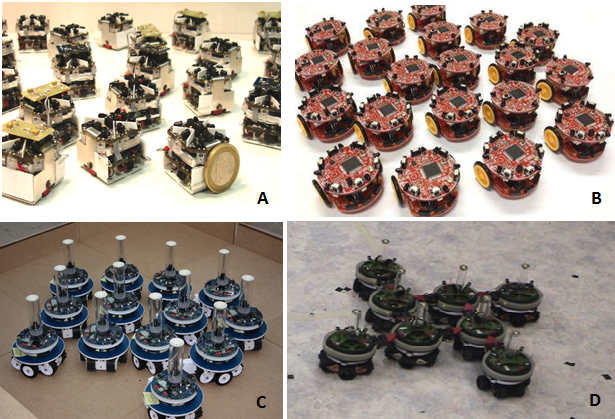
\includegraphics[scale = 0.7]{mobilerobots}
\end{figure}

    
    
  
    
Hou et al. has implemented a formation control system with dynamically changing formation shapes \cite{8}. Their approach defines a global objective function which requires the mathematical definition of the desired formation shape. But in real world applications it may not be possible to derive the analytical expressions for the desired shapes. In our work, control laws for individuals in the swarm does not require such a global objective function definition.

\begin{figure}[H]
\caption{Dynamical Formations with Global Objective Functions \cite{8}}
\centering
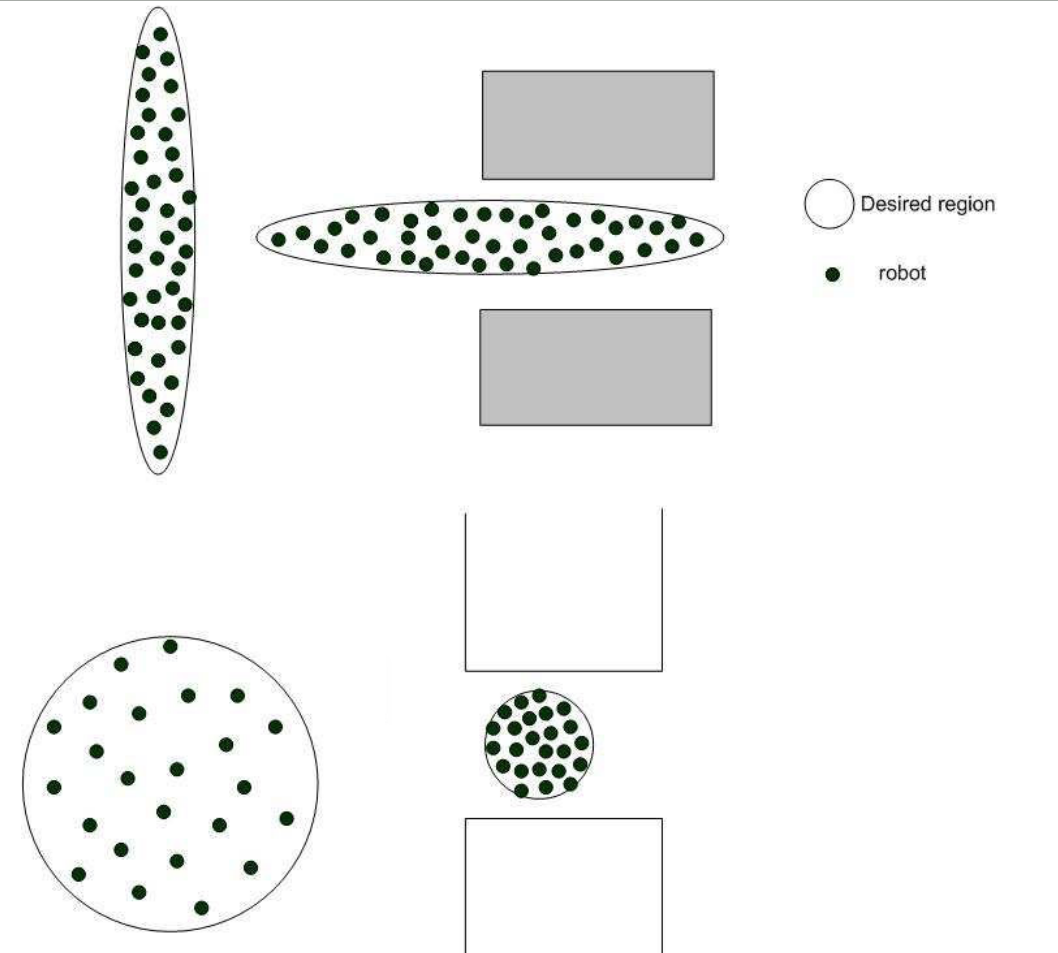
\includegraphics[scale = 0.32]{houslotine}
\end{figure}


\section{Objectives $\&$ Goals} \label{Objectives}
In this thesis work, our aim is to provide different approaches $\&$ solutions to the requirements in formation control problem.  There are mainly different types of  infrastructures which propose solutions to the formation control problems like the heterogeneity vs. homogeneity of the agents, communication structures, centralized vs. decentralized structures, swarm control strategies like behaviour based and leader-following approaches or virtual structure based approaches. 

Our main approach is to design a complete solution to the formation control problem by taking into account the requirements related with real world applications. In literature, formation control systems generally implements solutions with simple geometrical shapes \cite{8}. One of the objectives of this thesis work is to implement a solution which does not require the mathematical definition of the desired formation shape. Also it is aimed to design an algorithm which can adapt itself to the dynamically changing formations.

On the other hand, most of the related work assumes that it is possible to measure the exact positions of the agents in the workspace \cite{98,97}. Another objective of this thesis work is to implement a localization solution for the agents by assuming they may not able to measure their positions. With this approach, it is possible to provide a complete solution to the formation control problem.

Specific tasks including different missions, requires agents with different capabilities and this kind of tasks may not be achieved with swarms composed of homogeneous agents \cite{99}. In our work, one of the objectives is to implement a formation control system with heterogeneous agents. Furthermore, proposed solutions for formation control problem generally includes a decision making process which is executed by an individual agent or a central server. This kind of approach creates a single point of failure system and if this decision maker unit fails during mission, swarm cannot achieve the desired task. In this thesis work, it is aimed to implement a solution in which every agent is responsible of contributing on decisions and reaching a global consensus. 

In addition to choice of the formation control infrastructures, capabilities of the individual agents provide additional requirements and constraints while designing a formation control system. One of the most important characteristic of an agent in the swarm is its simplicity and limited sensor $\&$ communication capability \cite{6}. This approach results from the idea of achieving collective tasks with lots of simple individuals  and it is based on biological inspirations in nature like colonies of ants etc. In our work, it is aimed to propose a solution by taking into account that agents in the swarm has simple structures and limited sensor capabilities.

To achieve these objectives and meet these requirements, the goals for this thesis work are defined in the following subsections of \ref{Objectives}.

\subsection{Heterogenous Robots with Different Dynamics}
It is aimed to create a formation control system with heterogeneous agents to achieve complex tasks which require different functionalities. To accomplish this objective, it is assumed that agents have different dynamics from each other like different friction surfaces, geometrical structures, dynamics and functionalities. They have different volumes and masses and they may collide with the other ones and the obstacles in the environment.


\subsection{Communication Infrastructure}
One of the objectives in this work is to implement a localization solution for the agents. Also it is required to implement a communication backbone to execute a decentralized decision making process in which each agent reaches a global consensus. To meet these requirements, it is needed to implement a communication infrastructure in the proposed solution. By taking into account that the agents in the swarm have limited communication capabilities and can only negotiate with its local neighbors in a narrow line of sight range due to power consumption issues and their weak radio links, this infrastructure must have following specifications.

\begin{figure}[H]
\caption{Radio Links on Agents Have a Narrow LOS Range}
\centering
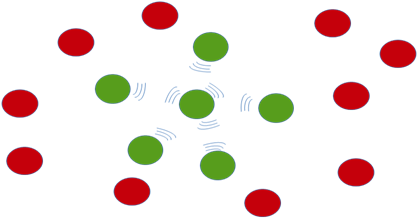
\includegraphics[scale = 1]{narrow_los}
\end{figure}

a)Communication Topology \newline
Communication topology is a wireless mesh network in which each agent relays data for the rest of the network. The network is fully connected and has routing technique where the data is propagated along a route by transporting over the nodes(member agents of the swarm).

\begin{figure}[H]
\caption{Mesh Network Between Agents}
\centering
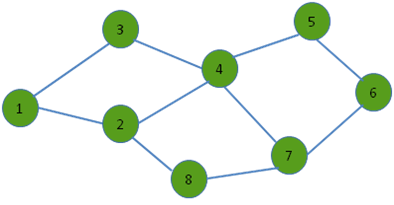
\includegraphics[scale = 1]{mesh}
\end{figure} 

b)Communication Bandwidth \newline
Bandwidth of the communication between agents is limited and nodes can only transport most critical data like heartbeats, agent IDs, type and position etc.

\subsection{ Decentralized Decision Making Process} \label{decent_decent}
Centralized formation controller systems implement a single controller  server/root node to process all the data needed to achieve the desired objectives. This type of systems achieve superior performance and optimal decisions  but they require high computational power, high communication bandwidths and are not robust due to dependence on a single controller \cite{12}. Decentralized formation controller structures have agents which are completely autonomous and responsible their own individual decisions. In this work, a hybrid centralized/decentralized controller architecture in which there is a central manager which partitions the desired formation shapes into goal states. Agents report their costs to reach these goal states and try to reach a consensus about final goal states to minimize the total displacement of the swarm.

\begin{figure}[H]
\caption{Agents Reach a Global Consensus on Goal States}
\centering
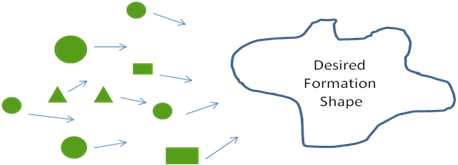
\includegraphics[scale = 0.8]{decentralized}
\end{figure} 

\subsection{Complex and Dynamically Changing Formation Shapes}
In literature, formation control systems are generally designed with a single or combination of simple geometrical shapes and they require analytical expressions of these shapes while implementing the proposed control laws for individual agents \cite{93}. Specific tasks which requires more complex shapes cannot be achieved with this approach. In our work, we have focused on designing a formation control algorithm which does not require the mathematical definition of the desired formation shape. The goal to accomplish this objective is to design a solution which does not depend on the analytical expression of the formation shape. Furthermore, in literature the general approach is to implement a solution to cover a static formation shape. In real world applications it may be needed to update the desired shape dynamically according to the requirements of the task. In our work, one of the goals is to propose an algorithm which can adapt itself to dynamically changing formation shapes.

\begin{figure}[H]
\caption{Complex and Dynamically Changing Formation Shapes}
\centering
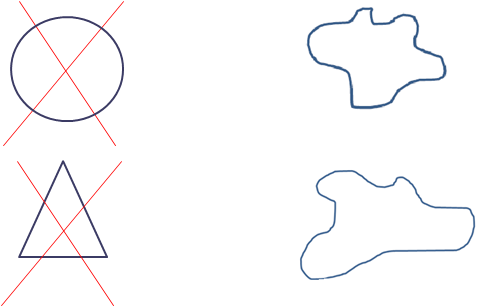
\includegraphics[scale = 0.7]{complex}
\end{figure}

\subsection{Simple Agents with Low Sensor Capabilities and Low Computing Powers}
In this project, we have assumed that the agents have low sensor capabilities and weak computing power \cite{6}. These constraints must be taken into account during the control system design, since individuals do not have a high resolution and sensitive data about the workspace and their states, and they cannot execute high level complex control algorithms.

\section{Requirements}
The goals of this project define some requirements about the implementation of the formation control system. These requirements are listed as follows:

1. Agents have to propagate their positions and velocity states with the help of inertial measurements.This process is handled with a Kalman estimator which takes the translational acceleration data as an input to the observer model .The translational acceleration data is calculated with the help of inertial measurements. 

2. Agents have to update$\&$adjust their position data with the help of agents which have positioning sensors(we call these agents position beacons) by local trilaterations.This position data is used in the estimator system as an external measurement to correct the drifts caused by propagation error of translational accelerations.

3. Agents have to update their route tables to create a communication backbone with the mesh network topology. Since agents are assumed to have low range$\&$bandwidth radio links, the propagation of a data between each agent in the swarm will be handled over this mesh network. 

4. Desired formation shape will be partitioned into potential goal states for different types of agents in shape partitioning based approaches. Performance analysis on proposed shape partitioning methods have to be done with some different criterias. 

5. Assignment of the agents to their target goal states should be done to minimize the total displacement of the agents while travelling towards the desired formation shape in shape partitioning based approaches. 

6. Simulations should be performed to compare the efficiency of different methods proposed in this thesis work. Different types of agents have to be represented with different dynamical and physical models during simulations.

7. Hardware demonstrations should be performed to illustrate the applicability of the proposed solution in real time systems. These applications may not contain the full implementation of the proposed system, but they must demonstrate a proof of concept(POC) environment.

\section{Methodology}
During the first part of the project, a local positioning system(LPS) is designed. In this system, agents which does not have position sensors, propagate their position and velocity states with their inertial measurements. Due to  drift problems on this solution \cite{91}, a position update process is handled with the help of local trilateration process. During the update phase of the solution, route tables for individual agents are determined with the help of Destination-Sequenced Distance Vector Routing Protocol (DSDV) algorithms. This process provides the required information to the agents about the position beacons which are their direct neighbors in the swarm. Position measurements are handled for each agent by local trilateration process with the help of position beacons which are direct neighbors of them. A Kalman observer is designed to fuse these propagation and update phases of the solution.

On the second part of the thesis work, formation control system is designed with two novel methods based on Bubble Packing method and Randomized Fractals method. Desired complex formation shapes are partitioned into goal states according to the heterogeneous agents in the swarm for both of these two methods. Decision process of the agents about their target goal states to minimize the total displacement of the swarm is implemented with the help of Visibility Graphs and Hungarian algorithms. Internal velocity controllers for individual agents to reach the goal states are implemented with a full state feedback method by regulating the augmented dynamical system with the gains optimized by Linear Quadratic Regulators (LQR).

\section{Contribution of Thesis}
The main contributions of thesis are:

1. Designing a local positioning system(LPS) based on local trilaterations to provide position data to the agents which do not have specific position sensors on their boards.

2. Implementing a wireless mesh network between agents in the swarm and designing a communication infrastructure and related routing algorithms to exchange the local data globally in the network

3. Implementing a formation control system with complex and dynamically changing formation shapes by using swarms composed of heterogeneous agents.

4. Designing and implementing the rules$\&$algorithms for the decentralized decision making process of the individual agents about the goal states in desired formation shape.


\section{Outline of the Thesis}
This thesis work is organized into 6 main sections. Chapter 1 introduces the main theme and the potential usage areas of formation control, while specifying our motivation and the requirements$\&$problems to meet$\&$solve related with the topic.

Chapter 2 gives literature reviews about the related works and discuss about the advantages$\&$disadvantages of the proposed method.

Chapter 3 introduces the methods and solutions used in two different parts of the problem; local positioning system and formation control system. In this chapter, routing algorithms and mathematical aspects of the trilateration process is introduced. On the other hand methods$\&$algorithms used for formation control is discussed in details.

Chapter 4 provides simulation analysis on the local positioning system and gives mutual evaluations of the performances of different methods used in formation control system.

Chapter 5 provides and discuss the details of hardware implementations and the experimental results.

Chapter 6 concludes the thesis and defines the future works related with the thesis.

% CHAPTER 2

\chapter{LITERATURE SURVEY}
\label{chp:Literature Survey}

\externaldocument{chapter1}
\externaldocument{chapter6}
\externaldocument{chapter3}
\externaldocument{chapter4}
\externaldocument{chapter5}

Formation control requires local positioning, detection of the general shape, task allocation to individual agents and task dispatching. The literature has related works in these different fields but lacks the dynamically formation control to dynamically changing shapes. This chapter is intended to motivate the need for the topic of this thesis by underlying the gap it filled by reviewing existing works in related fields. 
\section{Local Positioning Systems} \label{LPS_systems_ref}

Positioning systems are used to provide the required position data$\&$feedback to the systems where it is desired to control the location of the mobile agent in the workspace. 
These systems fall in to two main branches, global positioning systems and local positioning systems. Global positioning systems(GPS) has become increasingly popular for a couple of last decades for tracking location. In outdoor formation control applications this solution is used for positioning \cite{29}. It is a precise system depends on satellite based positioning mainly developed for direction finding and navigation.  Some of the problems encountered with the usage of GPS systems: (1) the signal from the satellites cannot penetrate to the indoor space so it doesn't perform in such areas, (2) it looses its precision in rich scattering environments such as urban areas \cite{19}.  A local positioning system can provide a position information where GPS systems are unavaliable,with the usage of signaling beacons which are placed at the exactly known locations. In indoor formation control applications this kind of approach is used for positioning \cite{96}. 




\begin{figure}[H]
	\caption{Accuracy Statistics of Different Positioning Sources \cite{20}} \label{overview_position}
	\centering
	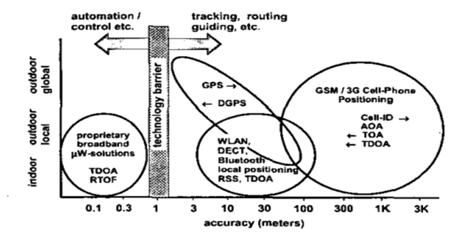
\includegraphics[scale = 0.4]{gps}
\end{figure} 

Figure \ref{overview_position} represents an overview of current positioning systems \cite{20}. Global positioning systems are widely used nowadays and they provide accuracies in the range of 3-30 meters. They further can operate in outdoor environments requiring radio signals from satellites. Differential GPS systems decrease these accuracy range below 3 meters with the help of additional local static beacons. GSM based solutions have the worst accuracy performance because they localize the nodes in the network by checking the relative signal strengths from different beacons, but they can perform in indoor environments partially \cite{20}.  Local positioning systems have the capability of working indoor environments because they use the signaling beacons which are placed at the exactly known locations \cite{20}. 

Local positioning systems has different system topologies illustrated in the Table \ref{different_top}20].

\begin {table}[H]
\begin{center}
\newcommand{\wrap}[1]{\parbox{.40\linewidth}{\vspace{1.5mm}#1\vspace{1mm}}}
\caption {Local Posititioning Systems with Different System Topologies \cite{20}} \label{different_top} 
\begin{tabular}{ |c|c| } 
\hline
\wrap{Concept} &\wrap{Concept	Definition} \\
\hline
\wrap{Remote Positioning} &\wrap{Measurement from remote site to mobile device}\\
\hline
\wrap{Self Positioning}&\wrap{Measurement from mobile unit to usually fixed transponders(landmarks)} \\
\hline
\wrap{Indirect remote positioning}&\wrap{Self positioning system with data transfer of measuring result to remote site } \\
\hline
\wrap{Indirect self positioning}&\wrap{Remote positioning system with data transfer of measuring result to mobile unit} \\			
 \hline
\end{tabular}
\end{center}
\end{table}

Two main topologies are self positioning and remote positioning systems \cite{20}.  In self positioning system a mobile device finds its own position with the help of a predetermined reference such as a starting point or a beacon node with exactly known positions. On the other hand, in remote positioning systems a mobile node locates other objects positions relative to its own position \cite{19}.   These two type of topologies can be converted to each other with the help of a communications structures integrated on the devices to share the result of position measurement and thus indirect remote positioning and indirect self positioning system topologies can be implemented. Self positioning systems can be implemented to provide position data to the individual agents in formation control problems. The approach is to distribute the position data to the individual agents from a beacon node with exactly known positions. The individual agents which do not have a positioning sensor on their boards, measure their distance to these beacons and correct their position data with these external measurements. Beacons are assumed to have a GPS sensor on their boards for outdoor applications. They are assumed to have a special tag to locate them in an indoor environment with the help of external devices such as E/O camera.




\subsection{Measurement Principles} \label{sssec:num1}
Local positioning systems are most relevant to formation control using robot networks. These systems differ mainly based on their measurement approaches which are the angle of arrival (AOA), received signal strength(RSS) and propogation-time based systems are commonly used as three different measurement techniques used in local positioning systems. 

\begin{figure}[H]
	\caption{Different Measurement Principles \cite{20}}
	\centering
	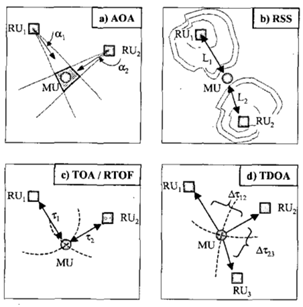
\includegraphics[scale = 0.4]{measurement}
\end{figure} 

In Angle-of-arrival (AOA) systems use directional antennas to measure the bearing and the angle to the points located at known positions are measured. The position value of device can be calculated with the intersection of several measurement, but the accuarcy is limited by shadowing and multipath reflections of radio signals \cite{20}. 

Received signal strength(RSS) systems calculate the distance value by taking the difference of the received signal power from the transmitted power. Some advanced propagation models are required to calculate the distance from the transmission loss in the air to eliminate the multipath fading and shadowing effects \cite{21}. 

Time based systems calculates the distance between measuring unit and signal transmitter with the help of propagation time like used in the global positioning systems generally. This process requires a perfect time synchronization between the mobile and stationary units \cite{20}.

In this thesis work, we implement a self positioning system in which every agent localize itself with the help of position beacons in the swarm with exactly known positions. The distance from the agents to these beacons in the swarm are assumed to be calculated with the help of a time of arrival(TOA) solution in which a node can calculate its distance to the transmitter beacon by measuring the difference between the timestamps of transmission and reception of the signal. 


\subsection{Trilateration Process} \label{Trilateration_Process_ref}

Trilateration process is used to determine the three dimensional position of unknown locations with the help of distance measurement to known positions \cite{22}. In self positioning systems, the main approach is to calculate the position of mobile agents with the help of distance measurements to the beacons with exactly known positions. This position calculations are handled with trilateration process. It is widely used in wireless sensor network topologies and local positioning systems.  In theory, it is needed to have at least four beacon nodes to calculte an unknown position in 3D, and at least three beacon nodes to calculate an unknown position in 2D environment. But these worst case numbers are generally not sufficient to estimate an unknown position with a good accuracy due to errors on range calculations and synchronization problems. Figure \ref{trilateration_ref} demonstrates a simple trilateration procees in 2D environment with the help of  three position beacons. Suppose a mobile device which tries to estimate its position with the help of local positioning system is at the red point in the figure. If it can measure its distance to the beacons named A,B and C with exactly known positions, it will be possible to estimate the unknown position of this mobile device with the same approach used in global positioning systems. 


\begin{figure}[H]
	\caption{Trilateration Process \cite{101}} \label{trilateration_ref}
	\centering
	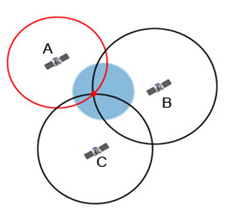
\includegraphics[scale = 1]{trilateration}
\end{figure}



\section{Formation Control Systems}
Formation control problem have different subproblems like formation shape generation, formation reconfiguration$\&$selection and formation tracking \cite{12}.  
In formation shape generation, agents are expected to get a formation shape which can be defined by external commands or with some mathematical constraint functions \cite{16}.  One general approach is to consider artificial potential functions. Samitha and Pubudu \cite{17} have presented an artificial potential function method  based on the consideration of the problem as controlling for the positioning of a swarm into a shape, bounded by a simple closed contour. This approach results in deploying uniformly of swarm agents within the contour.  Their work provides analysis about the stability and robustness of the proposed system based on Lyapunov like functions. Figure \ref{samitha_obstacle} illustrates a simulation environment of a swarm getting the desired pentagonal like formation shape in presence of obstacles. Here the desired formation shapes is defined with an analytical expression and individual control laws for agent are composed with artificial potential functions using this analytical expression. 

\begin{figure}[H]
	\caption{Motions and Formation of the Agents in Presence of Obstacles \cite{17}} \label{samitha_obstacle}
	\centering
	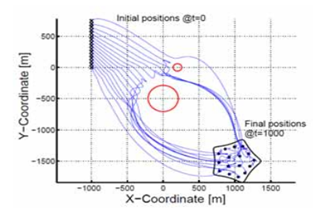
\includegraphics[scale = 0.7]{samitha}
\end{figure} 

In some applications, it may be needed to change the formation shape or splitting and joining of the agents together due to either a change in coordinated task requirements or change in environmental conditions such as narrow corridors. In such a scenario, the swarm has to propogate in a narrow corridor before reaching the desired goal state and it is not possible to follow this path by keeping the final desired formation shape. Hence, swarm has to adapt itself to environmental conditions while following a predetermined trajectory. This rask requires formation reconfiguration and dynamic task assignment of swarm agents to be dispatched. Hou and Slotine \cite{8} have defined a method based on global objective functions to provide formation control of a swarm agent. In their approach it is possible to implement scaling and rotating functions into control laws to adapt the swarm to environmental conditions while achieving a specific task. 

\begin{figure}[H]
	\caption{A Group of 100 Robots in a Rotating and Scaling Ellipse Formation \cite{8}} \label{slotine_fig_ref}
	\centering
	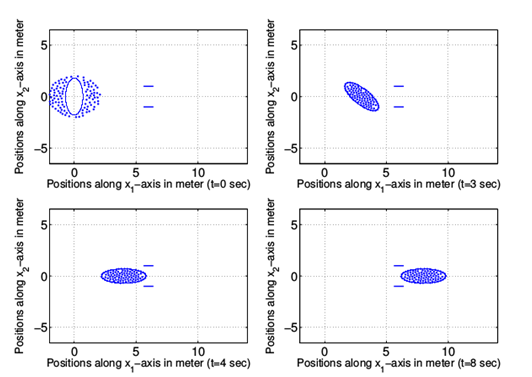
\includegraphics[scale = 1]{slotine}
\end{figure} 

Figure \ref{slotine_fig_ref} illustrates a simulation environment with a swarm of 100 mobile agents with an ellipsoidal formation shape. The formation shape is rotated dynamically to follow a path through a narrow corridor. Swarm has to adapt this  rotation maneuver to follow the desired trajectory. This kind of dynamical adaptations are always required in complex tasks in real time applications with complicated workspaces. 
One of the subproblems studied in formation control is formation tracking. The main objective of this problem is to maintain a desired formation with a group of robots, while tracking or following a reference trajectory. The solutions for the formation tracking approaches can be classified into three basic strategies as leader-following, virtual structure and behaviour based approaches \cite{12}. The most general strategy to provide a solution for this problem is leader-following swarm structures \cite{18}. Other strategies have a basis on optimization and graph theory approaches \cite{12}. Kumar, Fierro and Das proposed a vision based formation control framework  for this problem. This framework has a leader following infrastructure \cite{18}. Figure \ref{Kumar_Ferrro} illustrates a simulation environment of this leader follower approach on formation tracking problem. The individual agents achieve a coordinated turn by keeping their relative positions to their local neighbors. 

\begin{figure}[H]
	\caption{Five Robot Formation With Trajectory Tracking \cite{18}} \label{Kumar_Ferrro}
	\centering
	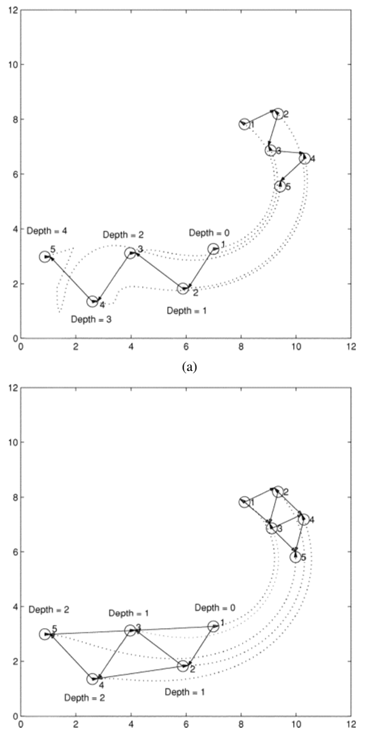
\includegraphics[scale = 0.65]{kumar}
\end{figure} 


In leader following strategy, some of the agents in the swarm are the leaders to manage the rest of the swarm to achieve a desired specific task and the rest of the agents act as followers. This approach reduces the formation control problem into tracking control problem of individuals to follow the leader from a desired distance and bearing angle, thus the stability and convergence analysis of the formation can be done with the usage of single tracking controllers of members thus simplifying the tracking problem of a network of agents to a single agent. Kumar, Fierro and Das at \cite{18} proposed a control framework in which follower agents move along a trajectory afterwords the leader agent with a desired separation distance $l_{ij}$ and desired relative bearing angle $\psi_{ij}$.  Figure \ref{leader_follower_ref} represents a formation control with three agents where R3 is the leader and R1,R2 are the follower agents. 

\begin{figure}[H]
	\caption{Leader-Follower Systems \cite{18}} \label{leader_follower_ref}
	\centering
	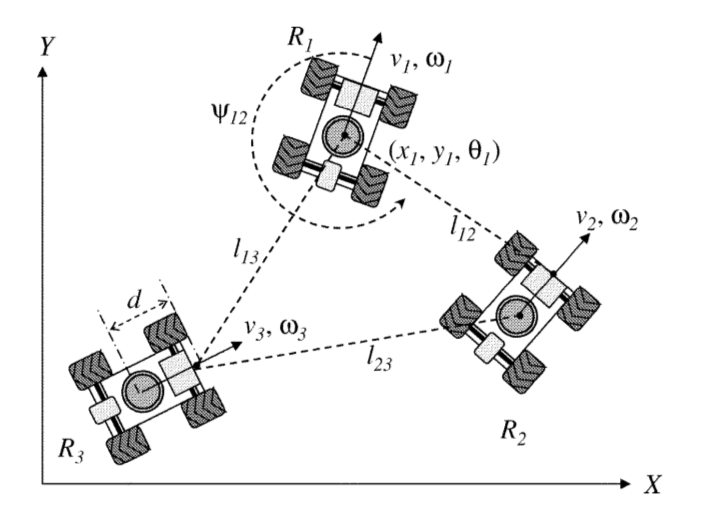
\includegraphics[scale = 0.5]{leader}
\end{figure}


In this approach it is hard to gather the agents in a certain shape. Another drawback is that, determining the separation and bearing angles for individual agents is getting harder as the number of agents in the swarm increases and this strategy is not fault tolerant to the absence of communication between agents.


In virtual structure approach, the formation is composed with a virtual rigid body. Formation control is applied to the whole virtual structure and then the individual agent control laws are determined with inverse dynamic solutions \cite{12}.  Lewis and Tan proposed a virtual structure based method for formation control in \cite{23} with a bidirectional flow control where robots move to stay in the virtual structure when the swarm is following a trajectory and virtual structure adapt itself to the robots' current positions to compensate the relative errors at the end of that maneuver. 

\begin{figure}[H]
	\caption{Maneuver of a Formation and Compensation of Virtual Structure}
	\centering
	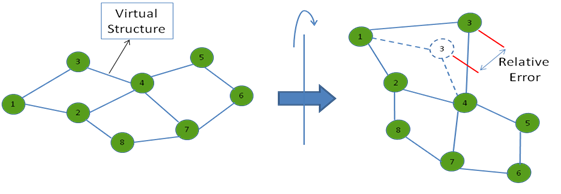
\includegraphics[scale = 0.95]{virtual_structure}
\end{figure}

In virtual structure strategy it is easy to achieve a coordinated behavior for the group to maintain the formation during a trajectory tracking or a maneuvering, but it is not a suitable strategy to apply a formation control to achieve certain geometrical shape with the swarm agents. 


Behavior based strategies model every agents' behaviors to achieve specific tasks with swarm. These behaviours may be very simple like randomly walk and avoidance of  obstacles in the environment or they may be defined in a very complicated manner in order to achieve complex formation shapes with the entire swarm while for example optimizing the overall energy consumption depending  upon the implementation of the controller structures.  One of the main usage of this strategy is artificial potential field based implementations . Cheng and Nagpal have introduced a robust and self repairing formation control method for swarms \cite{24}. In this approach, individual control laws for the agents are equipped with the artificial forces defined between agents themselves (to avoid collisions) and between the desired formation shape and agents. This solution provides robustness to the agent losses in the swarm during formation control and the rest of the swarm has the ability to refiil their absence in real time without changing the dynamics and the parameters of the formation controller. Because individual control laws are not dependent on the other member of the swarm. Each agent can calculate its own control input at an instant time with current formation shape and current members of the swarm and the whole swarm converge another equilibrium with current members \cite{24}. Figure \ref{izgara_ref} shows a simulation output of their work. Some of the agents from the right bottom corner of the desired formation shape are removed away from the swarm and the rest of the agents refill their absence during runtime. One of the main disadvantage of the artificial potential based approaches is that , the control forces applied to individual agents are determined instantaneously in accordance with that agent's and the other agents' positions and they cannot guarantee the optimization of the total distance travelled by the agents. Another drawback, related with this type of solution is that, there is a possibility to have local minimas in the solution where an agent reaches an undesired configuration point under the equilibrium of different types of artificial force components. In that case the total control input acting on the agent will be zero because of canceling force vectors which has opposite directions to each other generated by formation shape and obstacles etc. this strategy the solution may converge slowly to the steady state due to absence of generalized goal states for individual agents in the final state of formation. Because, there is no specific goal state for the individual agents to reach at the final configuration and they are expected to get a global equilibrium with the help of different artificial force components. 

\begin{figure}[H]
	\caption{Formation Control with Artificial Forces \cite{24}} \label{izgara_ref}
	\centering
	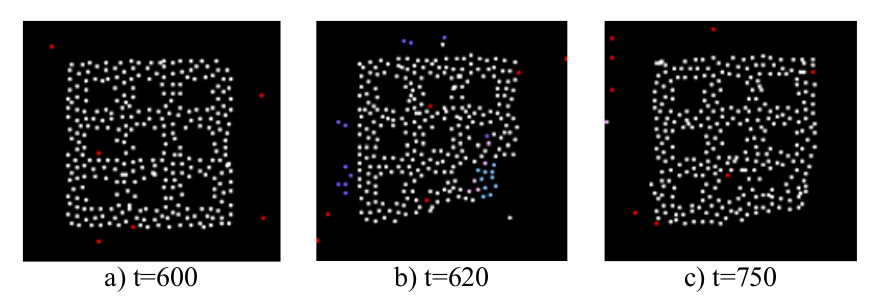
\includegraphics[scale = 0.4]{potential}
\end{figure}


Another approach is to define mathematical constraints and objective functions to achieve a specific formation shape by controlling the shape of the swarm colony while followinfg a trajectory.  Kumar and Belta \cite{25} presented an abstraction method of configuration space to a manifold defined as $A  = G x S$ where $G$ is a Lie group representing the position and the orientation of the swarm  and S represents the shape of the manifold.  They provide individual control laws which can be separately handled to manipulate the lie group $G$ to achieve formation tracking and orientation control and to manipulate the shape $S$ to achieve different geometrical shapes.Their method define the desired formation shape with shape manifold equations and control the orientation and the scale of this shape with lie group. Figure \ref{kumar_belta}
shows a simulation output in which the shape is defined as a rectangular area. The orientation and the scaling of the formation shape is dynamically changed to adapt the swarm different environmental conditions.Cheah and Slotine \cite{8} proposed a method based on objective functions . Common drawback for these researches, they can only implement a limited number of simple geometrical shapes because the desired formation shapes must be analytically identified on order to compose the related objective functions or shape manifolds. Even if it is possible to define a simple geometrical shape and to control the rotation and the scaling of this shape dynamically, there may be need for more complex and dynamically changing formation shapes rather than scaling and rotation maneuvers in real time applications. 



\begin{figure}[H]
	\caption{Formation Control with Objective Functions \cite{25}} \label{kumar_belta}
	\centering
	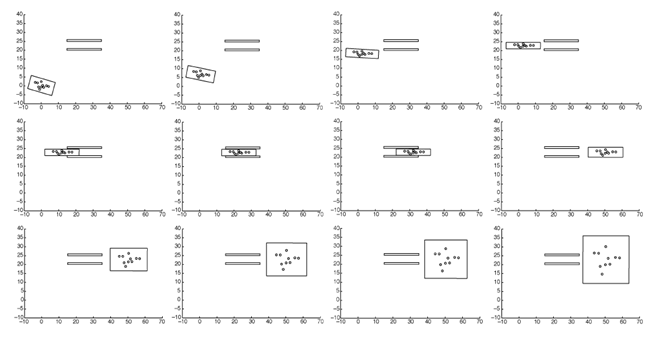
\includegraphics[scale = 0.8]{manifold}
\end{figure}



\section{Partitioning Complex Geometrical Shapes}

In this thesis work, one of the proposed solutions for the formation control problem is to partition the desired complex shapes into subsets of goal states for each type of agent in the swarm. Main idea is to dynamically assign the agents to these goal states on runtime to minimize the overall displacement of the swarm. Shape partitioning process is used to determine the goal states of the agents within the formation to cover the desired complex geometrical shape. There are some different solutions in the literature including fractal filling of space algorithms, bubble$\&$circle packing algorithms and advancing front algorithms. 

Fractals are self similar  patterns in all scales of themselves. They are defined with simple rules and they can cover any complex shape in the nature by progressing this simple rules iteratively. This approach is widely used in mesh generating algorithms and filling space problems.  Shier and Bourke \cite{26} have introduced a randomized fractal filling of space algorithm. They proposed a fractal based method to cover a given geometrical shape with the desired shapes and they provide the proof of their algorithm is space-filling with the following equations. Let $A$ be the total area to be filled. In our case, $A$ will be the area of the desired formation shape. If we choose the area of the fractals sequentially (i.e. bubbles which are representing the coverage area of the agents)  while filling the desired formation shape as $A_i$ with the following equation

	\begin{equation} \label{A_i_func}
	A_i = {\frac{A}{{\zeta(c,N)(i+N)^c}}}
	\end{equation}	
	
	where ${\zeta(c,N)}$ is the Hurwitz zeta function defined by 
	\begin{equation} \label{hurwitz}
	\zeta(c,N) = \sum_{i=0}^{\infty}\left(\frac{1}{(i+N)^c}\right)
	\end{equation}
	This Hurwitz zeta function will converge to zero while $i\to\infty$  with selection of $c>1$ and $N>0$. In view of Equation \ref{A_i_func} one can write by replacing the Hurwitz zeta function with the definition given in Equation \ref{hurwitz}
	\begin{equation} \label{A_i_equation}
	\sum_{i=0}^{\infty}A_i = \sum_{i = 0}^{\infty}\left(\frac{A}{\zeta(c,N)(i+N)^c}\right) = A
	\end{equation}


such that the sum of all areas $A_i$ is the total area $A$ to be filled, that is, if the algorithm does not halt then it is space-filling. Thus, it is possible to fill the desired shape with fractals chosen with areas defined in Equation \ref{A_i_equation}. Some of the outputs of their algorithm is given at Figure \ref{space_filling}. The desired shapes are filled with rectangular and star shaped fractals by selecting the areas as described in Equation \ref{A_i_equation}.



\begin{figure}[H]
	\caption{Space Filling Examples with Randomized Fractals \cite{26}} \label{space_filling}
	\centering
	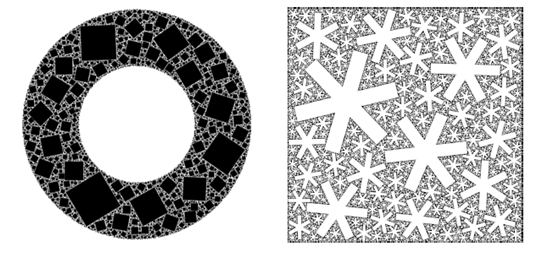
\includegraphics[scale = 1]{randomized1}
\end{figure}


Bubble$\&$Circle packing algorithms are widely used for mesh generation problems in finite element method. Shimada and Gossard \cite{27} proposed a method based on interbubble forces to provide close packaging of bubbles in desired geometrical shape. They define artificial interbubble forces to avoid collisions between bubbles and shape forces to keep the bubbles at the interior region of the desired shape. This idea is similar to the potential field based approaches in formation control problem since they both define artificial force components on individuals to cover a desired shape homogenously. The related interbubble forces are described at Figure \ref{interbubble_ref}. These forces have a nonlinear function of distance between the center of each bubbles and if this distance is larger than $l_o$, the interbubble forces are negative which means they attract each bubble towards the other ones. Interbubble forces increase while the distance between bubbles are decreasing to provide collision avoidance between bubbles. $l_o$ is the stable distance in which there is no interbubble force acting on bubble and it reaches an equilibrium point in the workspace.

\begin{figure}[H]
	\caption{Interbubble Forces \cite{27}} \label{interbubble_ref}
	\centering
	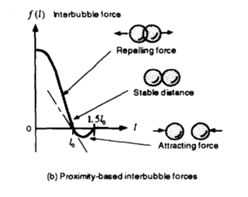
\includegraphics[scale = 0.3]{interbubble}
\end{figure}

The main idea is provide a close packing of bubbles which mimics a pattern of Voroni tessellation, corresponding to well shaped Delaunay triangles or tetrahedras.Figure \ref{tetrahedra} shows the corresponding voronoi polygons and delaunay triangles of a set of packed bubbles. The center of the cells in voronoi polygons are selected as the centers of the bubbles. Delaunay triangles corresponding to the set of uniformly packed of bubbles are well-shaped triangles \cite{27}. 

\begin{figure}[H]
	\caption{Uniform and Non-Uniform Node Spacing \cite{27}} \label{tetrahedra}
	\centering
	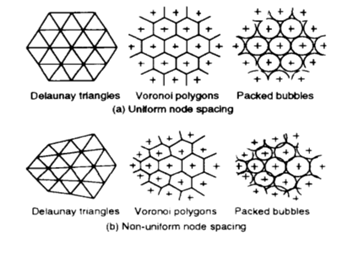
\includegraphics[scale = 0.35]{nodespacing}
\end{figure}

With the help of these interbubble forces, they provide an adaptive bubble packing algorithm for mesh generation. A result with a 2D shape is given at Figure \ref{mesh_genearation_ref}. At the end of 50 iterations, bubbles cover the desired shape with uniform spacing with the help of interbubble forces and the resultant delaunay triangulation corresponding to the set of packed bubbles are well-shaped triangles. 


\begin{figure}[H]
	\caption{Mesh Generation with Interbubble Forces \cite{27}} \label{mesh_genearation_ref}
	\centering
	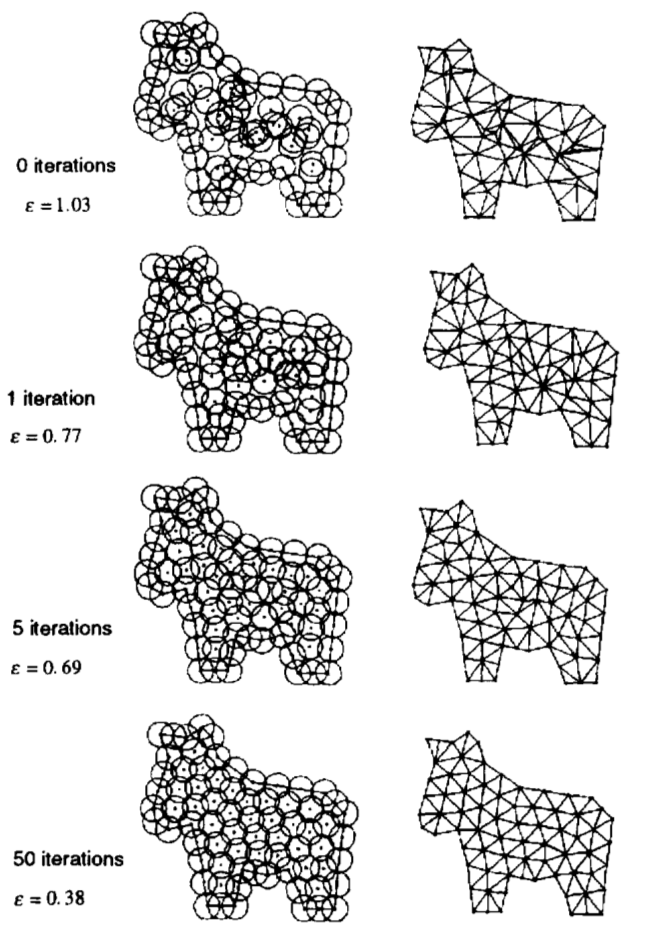
\includegraphics[scale = 0.4]{interbubble2}
\end{figure}

This approach can easily be augmented for different types and number of shapes to partition a complex geometrical shape with regular sets. It is possible to generate a mesh with different shapes which represents different types of agents in the swarm, rather than using bubbles with same radius. With this adaptation on the proposed method, it is possible to partition the desired shape into goal states which are subsets of different types of agents in the swarm with the help of interbubble forces. 

Advancing front methods are one of the alternatives used in mesh generation in literature.  In a two dimensional advancing front method, new triangles are added into the domain from the initial front boundary and the front is propogated iteratively between the meshed and the unmeshed region. The initial front is created by the desired outer boundary of the shape and the procedure continues until the given domain is fully meshed. 


\begin{figure}[H]
	\caption{Triangulation with Advancing Front Method \cite{103}}
	\centering
	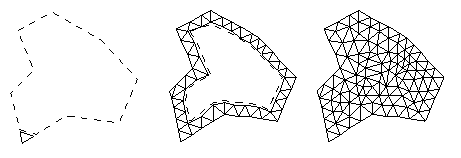
\includegraphics[scale = 0.65]{advancing}
\end{figure}



\chapter{Next Chapter}
This is another chapter. All these chapters can go into seperate .tex files and you can include
them with \verb|
% CHAPTER 1

\chapter{INTRODUCTION}
\label{chp:introduction}

This thesis work focuses on dynamic adaptation to achieve changes in formation of swarms consisting of heterogeneous mobile robots. The term of swarm has a meaning \cite{4}, a large group of locally interacting individuals with common goals. 

Self organizing swarm researches and its applications are generally inspired from the biological systems existing in the nature. Behaviours of complex biological systems remained unresolved for a long time, until recent researches that showed individuals with supple functionalities can achieve complex tasks by cooperation \cite{2}. Biological systems (such as colonies of ants) have simple behaviours but they can accomplish very complicated collective tasks in nature quite impossible to be achieved solely by individual capabilities. Beni \cite{1} describes this collaboration of members as follows:

Collaborative robot network is not just an agglomeration of robots, they have essential characteristics, which are found in swarms of insects, that is, decentralised control, which does not require synchronisation, and individuals which are simple and (quasi) identical.

Properties of swarm robotics systems that make them unique are the simplicity of individuals, restricted sensing and communication capabilities, collaborative achievement of complex tasks, robustness and decentralization of control capabilities \cite{6}.

Swarm robotics has been studied to produce different collective behaviours to solve different tasks such as as aggregation , pattern formation , self-assembly and morphogenesis , object clustering, assembling and construction , collective search$\&$rescue and exploration , coordinated motion , collective transportation , self-deployment , foraging and others\cite{5}. Dorigo and Trianni \cite{7} are studied on controllers for aggregation of coordinated motion of the identical mobile robots called swarm-bots. Their implementation has a centralized structure in which a decision maker assigns roles to individual agents. In our work, each agent is responsible to reach global consensus on the final positions in formation which increase the robustness of the system against to individual erroneous decisions. Hou et al. is focused on controlling of a swarm within a dynamically changing formation \cite{8}. In their work, it is needed to describe a global objective function which requires analytical expression of the desired formation shape. But it may not be possible to define the desired formation shape with analytical expressions in real world applications. In this thesis work, the solution does not require the analytical expressions of the desired formation shape.  Ganesh and Lisa introduced two new strategies for collective search and exploration of fields with swarm intelligence \cite{9}. Their implementation requires a central controller to manage the individuals and this type of solution has a single point of failure system characteristic because of the dependence on single decision maker agent.   Chaimowicz and Campos proposed a new methodology which is based on a dynamic role assignment mechanism in which the robots cooperate with each other and they demonstrate this method in a cooperative transportation task \cite{10}. Their work implements a leader follower structure in which following agents has no impact on the global consensus of the swarm. This approach depends on the decisions of an individual agent and an erroneous decisions of this individual may cause the failure of whole swarm. 

There are lots of studies related with different problems in swarm robotics literature as discussed briefly. In this thesis project, we are focused on dynamic pattern formation control of swarms consist of heterogeneous robots. All agents contribute on the decision process and they collaborate to minimize the total displacement while achieving the desired formation shape. 

\section{Problem Definition}
In this thesis work, we aimed to design a formation control system with heterogeneous robots and dynamically changing complex shapes. Desired formation shapes for real time applications, such as covering an area or a search$\&$rescue operation, may not be simple geometrical shapes with analytical expressions. The solution which does not require a mathematical definition of the desired formation shape is more suitable for these type of applications. On the other hand, this formation shape may be dynamically changing to meet the requirements of the task in real time. 

In literature, formation control systems generally include a decision making process which is executed by an individual agent or a central server. This kind of approach creates a single point of failure system and this ruler may cause a failure for the whole swarm by making a mistake. In this work, it is aimed to implement a solution in which each member of the swarm contributes on the decisions and global consensus of the swarm.

Formation control systems which are implemented with swarms composed of homogeneous agents cannot achieve special tasks which requires different functionalities of individual agents. In this work, we have focused on implementing a solution with a swarm consisting of heterogeneous agents with different capabilities. 

In this work, the main idea is to propose a complete design solution to a dynamically changing formation system, including a local positioning and formation control system. Formation control system heavily depends on the position data of individual agents in the workspace. Since it is expected to have high number of agents in the environment due to the nature of a swarm, the agents are assumed to have simple structures with low capabilities including lack of certain types of sensors. On the other hand, for indoor applications it will not be possible to use satellite dependent positioning systems on agents \cite{19}. Even if a positioning solution provided for an indoor application by different methods including visual feedback(by image processing), RSS(received signal strength) etc. , it is not possible to implement this solution for each single agent in the environment due to the increasing complexity and the costs by the number of agents. In literature, formation control systems are generally designed with the assumption of the positions of each agent is known exactly. To propose a complete solution for the formation control problem, it is required to implement a localization solution for the agents to provide the corrected positions in the workspace which will be used by the formation control system. This localization process must implement a solution to correct the position data of the agents within an maximum error bound. This error bound is determined by the requirements of the formation control problem. 

\section{Motivation}
The formation control problem is defined as the collaboration of a group of agents towards maintaining a formation with a certain shape \cite{12}. It focuses on leading the individual agents of a swarm to perform  collective tasks including shape generation and formation reconfiguration while traversing a trajectory avoiding collisions. These kind of tasks are achieved with a large group of simple robots  that can cooperate with each other. Formation control of multi agent systems  is an actively growing research field.

Swarms which are used in formation control systems, can be composed of homogeneous or heterogeneous agents according to the requirements of the problem. The usage of the homogeneous agents increases the total impact and the coverage of the system in the environment. This kind of a swarm has an increased redundancy and is capable of resuming the current task in case of failures of some of the agents during mission. On the other hand, a swarm composed of heterogeneous agents has different capabilities of the agents. This kind of a system can be used in tasks which requires different functionalities has to be performed individually or simultaneously.

In real world applications there may be need for different  functionalities to achieve some specific tasks. If this is the case, one solution may be to design a sophisticated robot which includes all required capabilities for this task. In this scenario, this robot will be the single point of failure in the system and if robustness is a  vital feature for this solution, some redundant robots have to be added to the system. It is clear that the design of such an advanced robot and hold its redundant backups in the system will increase the cost of the solution. In swarm robotics concept, one of the approaches related with the usage of the heterogeneous agents is to gather some different types of simple mobile robots which have their own specific functionalities to achieve a collective task rather than designing an advanced robot for the solution \cite{99}. With this approach, the robustness of the system is increased, costs are reduced down and the reusability of the individual members of the swarm for other tasks is provided.  A project named Swarmanoid which is funded by European Commission, has an objective to implement and control of a novel distributed robotic system. The system is designed with heterogeneous, dynamically connected, small autonomous robots called foot-bots , hand-bots and eye-bots where foot-bots are responsible to transport the required materials(including other types of robots) to a specific task area and hand-bots are responsible for operations to be handled with their manipulators and eye-bots are responsible of observations and reconnaissance on the workspace. This project implements a system which has a leader follower structure in which a decision maker agent assign different tasks and roles to the other members of the swarm. Wrong decisions or the failure of this decision maker may prevent the whole swarm to achieve the desired task. In this thesis work, we have focused on a system in which each agent is responsible to contribute on the decision process.

\begin{figure}[H]
\caption{A Robot Team Consists of Eyebot, Handbot and Footbot Agents \cite{99}}
\centering
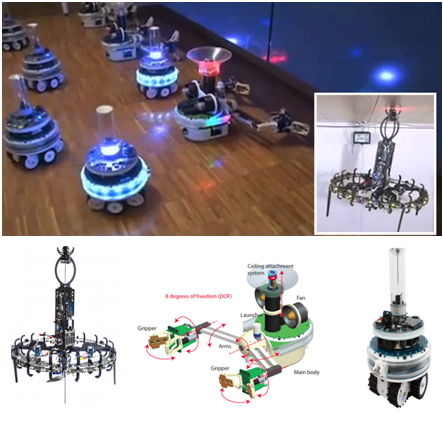
\includegraphics[scale = 1]{eyebot}
\end{figure} 
\newpage
A swarm which is composed with same type of homogeneous agents can be used to increase the total impact and the energy of an individual agent. This kind of a system can be used in missions like coverage, search and  reconnaissance etc.  Martin and Kilberg have worked on formation control and formation tracking of  microsatellites to achieve continuous coverage and improved capability. They also mentioned that small formations will reduce the fuel consumption for propulsion and expand the sensing capabilities of microsatellites \cite{15}.

\begin{figure}[H]
\caption{Sparse Aperture Formation of Micro Satellites \cite{15}}
\centering
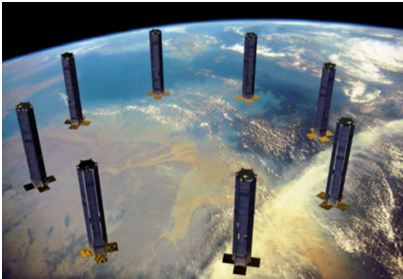
\includegraphics[scale = 1]{Satellite}
\end{figure} 

Formation control solutions has lots of usage areas such as coverage missions, security patrols and search$\&$rescue in hazardous environments etc.\cite{13}. For missions related with area coverage and reconnaissance, a group of autonomous vehicles may be required to keep in a specified formation \cite{13}.  

There are some hardware implementations to test the related formation control algorithms in real time applications. Since the formation control problem requires lots of agents in a swarm, these works have a common point of providing agents with minimal costs and sensor capabilities. The Kilobot Project from Harvard university have released their agents with the name of Kilobots and they have teams which are working on different formation control problems with Kilobots \cite{98}.

\begin{figure}[H]
\caption{Formation Control with Kilobots \cite{98}}
\centering
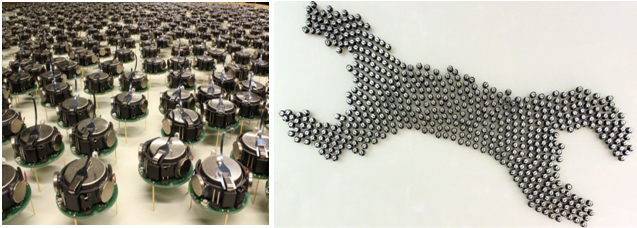
\includegraphics[scale = 0.70]{kilobot}
\end{figure}

These micro robots have a great reusability for different types of formation control problems  and they have biological inspiration from the nature in the sense of individual simplicity and power of collective behaviours. Common feature of these projects, they implement formation control systems with swarms composed of homogeneous agents. In real world applications, complex tasks may require different functionalities which can be provided by different types of robots. In our work, we have focused on implementing a formation control system with heterogeneous agents.

\begin{figure}[H]
\captionsetup{format=hang,justification=centerfirst}
\caption{
A) Swarm Robot Project from Universities of Stuttgart \cite{97}  \\
B) Colias Project from Lincoln University and Tsinghua University\cite{96}\\
C) Marx bot developed at EPFL\cite{95} \\
D)Swarm bots project conducted by  European Commission \cite{94}}

\centering
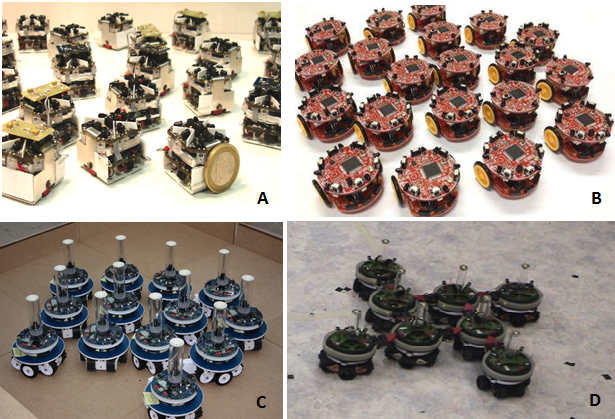
\includegraphics[scale = 0.7]{mobilerobots}
\end{figure}

    
    
  
    
Hou et al. has implemented a formation control system with dynamically changing formation shapes \cite{8}. Their approach defines a global objective function which requires the mathematical definition of the desired formation shape. But in real world applications it may not be possible to derive the analytical expressions for the desired shapes. In our work, control laws for individuals in the swarm does not require such a global objective function definition.

\begin{figure}[H]
\caption{Dynamical Formations with Global Objective Functions \cite{8}}
\centering
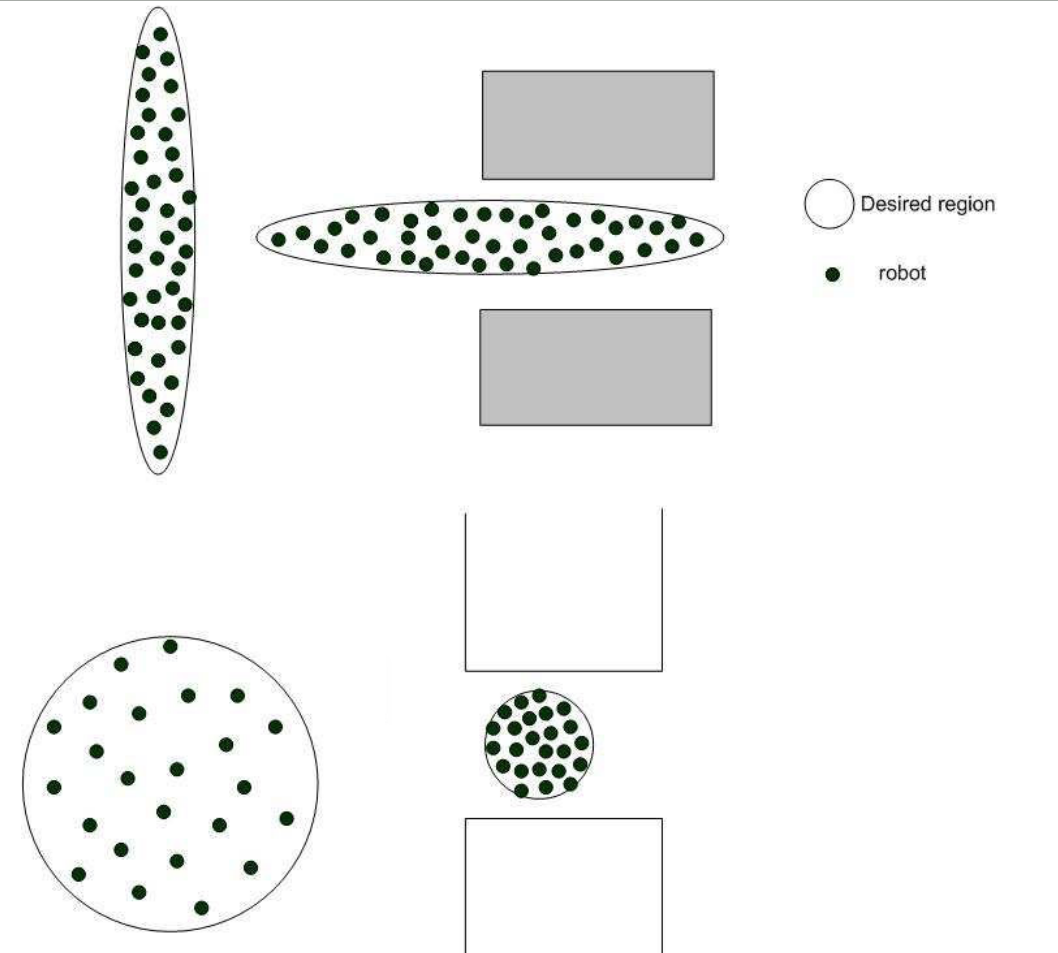
\includegraphics[scale = 0.32]{houslotine}
\end{figure}


\section{Objectives $\&$ Goals} \label{Objectives}
In this thesis work, our aim is to provide different approaches $\&$ solutions to the requirements in formation control problem.  There are mainly different types of  infrastructures which propose solutions to the formation control problems like the heterogeneity vs. homogeneity of the agents, communication structures, centralized vs. decentralized structures, swarm control strategies like behaviour based and leader-following approaches or virtual structure based approaches. 

Our main approach is to design a complete solution to the formation control problem by taking into account the requirements related with real world applications. In literature, formation control systems generally implements solutions with simple geometrical shapes \cite{8}. One of the objectives of this thesis work is to implement a solution which does not require the mathematical definition of the desired formation shape. Also it is aimed to design an algorithm which can adapt itself to the dynamically changing formations.

On the other hand, most of the related work assumes that it is possible to measure the exact positions of the agents in the workspace \cite{98,97}. Another objective of this thesis work is to implement a localization solution for the agents by assuming they may not able to measure their positions. With this approach, it is possible to provide a complete solution to the formation control problem.

Specific tasks including different missions, requires agents with different capabilities and this kind of tasks may not be achieved with swarms composed of homogeneous agents \cite{99}. In our work, one of the objectives is to implement a formation control system with heterogeneous agents. Furthermore, proposed solutions for formation control problem generally includes a decision making process which is executed by an individual agent or a central server. This kind of approach creates a single point of failure system and if this decision maker unit fails during mission, swarm cannot achieve the desired task. In this thesis work, it is aimed to implement a solution in which every agent is responsible of contributing on decisions and reaching a global consensus. 

In addition to choice of the formation control infrastructures, capabilities of the individual agents provide additional requirements and constraints while designing a formation control system. One of the most important characteristic of an agent in the swarm is its simplicity and limited sensor $\&$ communication capability \cite{6}. This approach results from the idea of achieving collective tasks with lots of simple individuals  and it is based on biological inspirations in nature like colonies of ants etc. In our work, it is aimed to propose a solution by taking into account that agents in the swarm has simple structures and limited sensor capabilities.

To achieve these objectives and meet these requirements, the goals for this thesis work are defined in the following subsections of \ref{Objectives}.

\subsection{Heterogenous Robots with Different Dynamics}
It is aimed to create a formation control system with heterogeneous agents to achieve complex tasks which require different functionalities. To accomplish this objective, it is assumed that agents have different dynamics from each other like different friction surfaces, geometrical structures, dynamics and functionalities. They have different volumes and masses and they may collide with the other ones and the obstacles in the environment.


\subsection{Communication Infrastructure}
One of the objectives in this work is to implement a localization solution for the agents. Also it is required to implement a communication backbone to execute a decentralized decision making process in which each agent reaches a global consensus. To meet these requirements, it is needed to implement a communication infrastructure in the proposed solution. By taking into account that the agents in the swarm have limited communication capabilities and can only negotiate with its local neighbors in a narrow line of sight range due to power consumption issues and their weak radio links, this infrastructure must have following specifications.

\begin{figure}[H]
\caption{Radio Links on Agents Have a Narrow LOS Range}
\centering
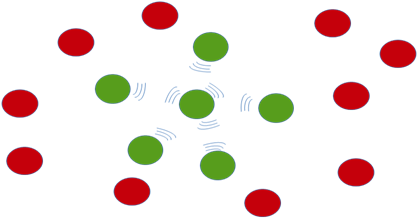
\includegraphics[scale = 1]{narrow_los}
\end{figure}

a)Communication Topology \newline
Communication topology is a wireless mesh network in which each agent relays data for the rest of the network. The network is fully connected and has routing technique where the data is propagated along a route by transporting over the nodes(member agents of the swarm).

\begin{figure}[H]
\caption{Mesh Network Between Agents}
\centering
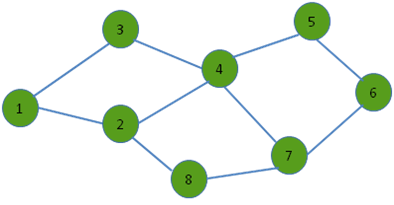
\includegraphics[scale = 1]{mesh}
\end{figure} 

b)Communication Bandwidth \newline
Bandwidth of the communication between agents is limited and nodes can only transport most critical data like heartbeats, agent IDs, type and position etc.

\subsection{ Decentralized Decision Making Process} \label{decent_decent}
Centralized formation controller systems implement a single controller  server/root node to process all the data needed to achieve the desired objectives. This type of systems achieve superior performance and optimal decisions  but they require high computational power, high communication bandwidths and are not robust due to dependence on a single controller \cite{12}. Decentralized formation controller structures have agents which are completely autonomous and responsible their own individual decisions. In this work, a hybrid centralized/decentralized controller architecture in which there is a central manager which partitions the desired formation shapes into goal states. Agents report their costs to reach these goal states and try to reach a consensus about final goal states to minimize the total displacement of the swarm.

\begin{figure}[H]
\caption{Agents Reach a Global Consensus on Goal States}
\centering
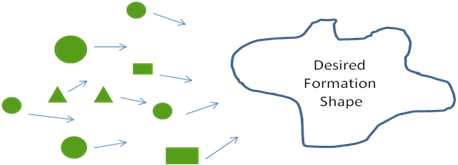
\includegraphics[scale = 0.8]{decentralized}
\end{figure} 

\subsection{Complex and Dynamically Changing Formation Shapes}
In literature, formation control systems are generally designed with a single or combination of simple geometrical shapes and they require analytical expressions of these shapes while implementing the proposed control laws for individual agents \cite{93}. Specific tasks which requires more complex shapes cannot be achieved with this approach. In our work, we have focused on designing a formation control algorithm which does not require the mathematical definition of the desired formation shape. The goal to accomplish this objective is to design a solution which does not depend on the analytical expression of the formation shape. Furthermore, in literature the general approach is to implement a solution to cover a static formation shape. In real world applications it may be needed to update the desired shape dynamically according to the requirements of the task. In our work, one of the goals is to propose an algorithm which can adapt itself to dynamically changing formation shapes.

\begin{figure}[H]
\caption{Complex and Dynamically Changing Formation Shapes}
\centering
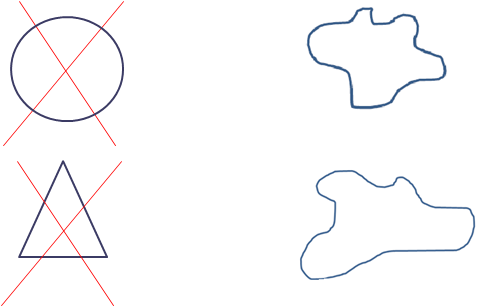
\includegraphics[scale = 0.7]{complex}
\end{figure}

\subsection{Simple Agents with Low Sensor Capabilities and Low Computing Powers}
In this project, we have assumed that the agents have low sensor capabilities and weak computing power \cite{6}. These constraints must be taken into account during the control system design, since individuals do not have a high resolution and sensitive data about the workspace and their states, and they cannot execute high level complex control algorithms.

\section{Requirements}
The goals of this project define some requirements about the implementation of the formation control system. These requirements are listed as follows:

1. Agents have to propagate their positions and velocity states with the help of inertial measurements.This process is handled with a Kalman estimator which takes the translational acceleration data as an input to the observer model .The translational acceleration data is calculated with the help of inertial measurements. 

2. Agents have to update$\&$adjust their position data with the help of agents which have positioning sensors(we call these agents position beacons) by local trilaterations.This position data is used in the estimator system as an external measurement to correct the drifts caused by propagation error of translational accelerations.

3. Agents have to update their route tables to create a communication backbone with the mesh network topology. Since agents are assumed to have low range$\&$bandwidth radio links, the propagation of a data between each agent in the swarm will be handled over this mesh network. 

4. Desired formation shape will be partitioned into potential goal states for different types of agents in shape partitioning based approaches. Performance analysis on proposed shape partitioning methods have to be done with some different criterias. 

5. Assignment of the agents to their target goal states should be done to minimize the total displacement of the agents while travelling towards the desired formation shape in shape partitioning based approaches. 

6. Simulations should be performed to compare the efficiency of different methods proposed in this thesis work. Different types of agents have to be represented with different dynamical and physical models during simulations.

7. Hardware demonstrations should be performed to illustrate the applicability of the proposed solution in real time systems. These applications may not contain the full implementation of the proposed system, but they must demonstrate a proof of concept(POC) environment.

\section{Methodology}
During the first part of the project, a local positioning system(LPS) is designed. In this system, agents which does not have position sensors, propagate their position and velocity states with their inertial measurements. Due to  drift problems on this solution \cite{91}, a position update process is handled with the help of local trilateration process. During the update phase of the solution, route tables for individual agents are determined with the help of Destination-Sequenced Distance Vector Routing Protocol (DSDV) algorithms. This process provides the required information to the agents about the position beacons which are their direct neighbors in the swarm. Position measurements are handled for each agent by local trilateration process with the help of position beacons which are direct neighbors of them. A Kalman observer is designed to fuse these propagation and update phases of the solution.

On the second part of the thesis work, formation control system is designed with two novel methods based on Bubble Packing method and Randomized Fractals method. Desired complex formation shapes are partitioned into goal states according to the heterogeneous agents in the swarm for both of these two methods. Decision process of the agents about their target goal states to minimize the total displacement of the swarm is implemented with the help of Visibility Graphs and Hungarian algorithms. Internal velocity controllers for individual agents to reach the goal states are implemented with a full state feedback method by regulating the augmented dynamical system with the gains optimized by Linear Quadratic Regulators (LQR).

\section{Contribution of Thesis}
The main contributions of thesis are:

1. Designing a local positioning system(LPS) based on local trilaterations to provide position data to the agents which do not have specific position sensors on their boards.

2. Implementing a wireless mesh network between agents in the swarm and designing a communication infrastructure and related routing algorithms to exchange the local data globally in the network

3. Implementing a formation control system with complex and dynamically changing formation shapes by using swarms composed of heterogeneous agents.

4. Designing and implementing the rules$\&$algorithms for the decentralized decision making process of the individual agents about the goal states in desired formation shape.


\section{Outline of the Thesis}
This thesis work is organized into 6 main sections. Chapter 1 introduces the main theme and the potential usage areas of formation control, while specifying our motivation and the requirements$\&$problems to meet$\&$solve related with the topic.

Chapter 2 gives literature reviews about the related works and discuss about the advantages$\&$disadvantages of the proposed method.

Chapter 3 introduces the methods and solutions used in two different parts of the problem; local positioning system and formation control system. In this chapter, routing algorithms and mathematical aspects of the trilateration process is introduced. On the other hand methods$\&$algorithms used for formation control is discussed in details.

Chapter 4 provides simulation analysis on the local positioning system and gives mutual evaluations of the performances of different methods used in formation control system.

Chapter 5 provides and discuss the details of hardware implementations and the experimental results.

Chapter 6 concludes the thesis and defines the future works related with the thesis.|. For only one citation \cite{bpeltools}, for multiple citations \cite{atkinson04,erl05,kitchenham07}.

\bibliographystyle{plain}	
%
% References in Bibtex format goes into below indicated file with .bib extension
\bibliography{thesis_references}
% You can use full name of authors, however most likely some of the Bibtex entries you will find, will use abbreviated first names
% If you don't want to correct each of them by hand, you can use abbreviated style for all of the references

\appendix
\chapter{Appendix Name}
Appendix content goes here.
 
%
% If you are a Ph.D. Student you need to insert a CV at the end of you thesis
% Check vita.tex for a simple CV template in Latex
\curriculumvitae
\label{chapter:vita}

\section*{\uppercase{Personal Information}}

\textbf{Surname, Name: } Çimenci, Kadir\\
\textbf{Nationality:} Turkish (TC) \\
\textbf{Date and Place of Birth:} 11.07.1988, Ankara\\
\textbf{Marital Status:} Single \\
\textbf{Phone:} 0 533 7229934 \\


\section*{\uppercase{Education}}

\begin{tabular}{lll}
\textbf{Degree} & \textbf{Institution} & \textbf{Year of Graduation} \\
B.S. & Electrical$\&$Electronics Engineering Faculty, ITU & 2012 \\
B.S. & Mechanical Engineering Faculty, ITU & 2012 \\
High School & Işıklar Askeri Lisesi & 2006
\end{tabular}

\section*{\uppercase{Professional Experience}}

\begin{tabular}{lll}
\textbf{Year} & \textbf{Place} & \textbf{Enrollment} \\
2 & Turkish Aerospace Industry, TAI & Design Engineer \\
2 & HAVELSAN & Embedded Software Engineer
\end{tabular}

%\section*{\uppercase{Publications}}
%\subsection*{International Conference Publications}
%Your publications goes here. Do not try to use Bibtex, since Bibtex builds a single %bibliography
%database for the document.

\end{document}
